%% LyX 2.3.1-1 created this file.  For more info, see http://www.lyx.org/.
%% Do not edit unless you really know what you are doing.
\documentclass[english,spanish]{article}
\usepackage[T1]{fontenc}
\usepackage[latin9]{luainputenc}
\usepackage{geometry}
\geometry{verbose,tmargin=2.5cm,bmargin=2.5cm,lmargin=25mm,rmargin=25mm}
\usepackage{verbatim}
\usepackage{float}
\usepackage{amsmath}
\usepackage{amssymb}
\usepackage{graphicx}
\usepackage{babel}
\addto\shorthandsspanish{\spanishdeactivate{~<>}}

\begin{document}
\selectlanguage{english}%
\begin{titlepage}
\newcommand{\HRule}{\rule{\linewidth}{0.5mm}}       
\center        
%---------------------------------------------------------------------------------------- 
%	HEADING SECTIONS 
%----------------------------------------------------------------------------------------      
\textsc{\LARGE Instituto Tecnol�gico de Buenos Aires}\\[2cm]  
\textsc{\Large 22.85 Sistemas de Control}\\[1.5cm]  
%\textsc{\large Trabajo Pr�ctico Final$ }\\[0.5cm]
%---------------------------------------------------------------------------------------- 
%	TITLE SECTION 
%----------------------------------------------------------------------------------------      
\HRule \\[0.5cm] 
{ \huge Trabajo Pr�ctico Final}
\\[0.4cm]  \HRule \\[2cm]       
%---------------------------------------------------------------------------------------- 
%	AUTHOR SECTION 
%----------------------------------------------------------------------------------------      
\begin{minipage}{0.4\textwidth} \begin{flushleft} \large 
\emph{Grupo 3:}\\		 [.3cm]
Ezequiel \textsc{Vijande}\\ Leg. 58057 \\  [.3cm] 
Lucero Guadalupe \textsc{Fernandez}\\ Leg. 57485 \\  [.3cm]
Manuel Fernando \textsc{Moll�n}\\ Leg. 58023 \\  [.3cm]
Mat�as Agust�n \textsc{Larroque}\\ Leg. 56597 \\  [.3cm]
Robin \textsc{Bertrand}\\ Leg. 61739 \\  [.3cm]
Tom�s Agust�n \textsc{Gonz�lez Orlando}\\ Leg. 57090 \\  [.3cm] 
\end{flushleft} \end{minipage} ~ 
\begin{minipage}{0.4\textwidth} \begin{flushright} \large 
\emph{Profesores:} \\ [.3cm] 
Victor Gustavo  \textsc{Nasini}\\
Cristian Alejo  \textsc{Zujew}\\
\end{flushright} \end{minipage}\\[2cm]      
%---------------------------------------------------------------------------------------- 
%	DATE SECTION 
%----------------------------------------------------------------------------------------      
\vfill {\large Entregado: 10 de Julio de 2020}\\[2cm]      \vfill       
\end{titlepage}\selectlanguage{spanish}%

\newpage{}

\section{Introducci�n}

El siguiente proyecto consiste en la realizacion de un sistema que
controle la altura a la que levita una pelota de ping pong dentro
de un tubo pl�stico. El controlador se realiz� utilizando PID digital
por medio de un arduino.

A lo largo de este informe se explicar� el modelo f�sico del problema,
la implementaci�n del controlador as� como los resultados del mismo.

\section{Objetivos y resumen}

El objetivo principal del proyecto es poder lograr que una pelota
de ping pong se mantenga a una altura constante dentro de un tubo
pl�stico a pesar de posibles alteraciones en la posici�n de la misma.

La planta de nuestro sistema consiste, como se mencion� previamente,
de un tubo pl�stico posicionado de manera vertical dentro del cual
se encuentra la pelota de ping pong. Para mantenerla en una misma
posici�n se cuenta con un ventilador en la base del tubo que levanta
la pelota, como tambi�n de un sensor infrarrojo en la parte superior
del tubo que censa la posici�n de la misma. La funci�n del Arduino
es controlar la velocidad del ventilador mediante control PID para
variar el flujo del aire y permitir que la pelota se mantenga estable.

Cabe aclarar que el tubo cuenta con ranuras laterales para permitir
el flujo de aire hacia el exterior proveniente del ventilador.
\begin{center}
\begin{figure}[H]
\caption{Imagen del sistema implementado}

\end{figure}
\par\end{center}

\section{Marco Te�rico}

Para el modelado f�sico del sistema se considera que s�lo act�an dos
fuerzas para la pelota que est� dentro del tubo, la fuerza del aire
que empuja a la pelota y la fuerza gravitacional.
\begin{center}
\begin{figure}[H]
\begin{centering}
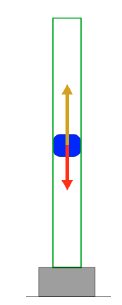
\includegraphics{Imagenes/Fisico.PNG}
\par\end{centering}
\caption{Diagrama de fuerzas de la pelota dentro del tubo}

\end{figure}
\par\end{center}

De la segunda Ley de Newton se tiene que:
\begin{center}
\[
m\frac{d^{2}y}{dt^{2}}=\sum F_{y}
\]
\par\end{center}

\begin{center}
\[
m\frac{d^{2}y}{dt^{2}}=F_{aire}-F_{g}
\]
\par\end{center}

\begin{center}
\begin{equation}
\frac{d^{2}y}{dt^{2}}=\frac{1}{2m}C_{d}\rho\pi r^{2}(v_{aire}-\frac{dy}{dt})^{2}-g
\end{equation}
\par\end{center}

Donde:
\begin{itemize}
\item $\rho\sim1.2kg/m^{3}$, la densidad volum�trica del aire
\item $m=2.7g$, la masa de la pelota de ping pong
\item $r=2cm$ es el radio de la pelota de ping pong
\item $y$ es la posici�n vertical de la pelota dentro del tubo
\item $v_{aire}$ es la rapidez promedio del aire cerca de la pelota
\item $g=9.81m/s^{2}$, la constante gravitacional
\item $C_{d}=\frac{24}{Re}+\frac{6}{1+\sqrt{Re}}+0.4$, el coeficiente de
arrastre
\item $Re=\frac{2r\rho(v_{aire}-\frac{dy}{dt})}{\eta}$
\item $\eta$ es la viscosidad din�mica del aire.
\end{itemize}
Asumiendo que $Re>1000$ ($C_{d}\thickapprox0.4$) lo cual es v�lido
si la pelota tiene un radio de 2cm y la velocidad del aire es mayor
a $0.66\frac{m}{seg}$. Entonces la ecuaci�n del problema resulta:
\begin{center}
\begin{equation}
\frac{d^{2}y}{dt^{2}}=\frac{1}{5m}\rho\pi r^{2}(v_{aire}-\frac{dy}{dt})^{2}-g\label{eq:Edo}
\end{equation}
\par\end{center}

Consideramos como la salida del sistema la altura de la pelota de
ping pong con respecto a la base con el ventilador, mientras que la
entrada del sistema es la tensi�n de continua que fija la velocidad
con la que gira el ventilador de la base. La variable $v_{aire}$
en la ecuaci�n \ref{eq:Edo} est� relacionada con la velocidad con
la que gira el ventilador mediante una funci�n matem�tica desconocida
$v_{aire}=f(y,V_{DC})$.

Debido a la complejidad del modelo, se decidi� obtener la transferencia
a lazo abierto del sistema de manera emp�rica a trav�s de un an�lisis
de la salida obtenida a partir de una determinada entrada cerca del
punto de equilibrio del sistema. Se puede ver de la ecuaci�n \ref{eq:Edo}
que el sistema no es lineal por lo que se eligi� como punto de equilibrio
la altura correspondiente a la mitad del tubo y se trabaja como si
el sistema fuera lineal cerca de dicho punto de equilibrio.

Encontrando la relaci�n lineal entre la tensi�n proporcionada al ventilador
y su velocidad resultante, es decir, algo de la forma $v_{aire}[m/s]=K_{a}.V_{DC}+cte$,
la ecuaci�n \ref{eq:Edo} quedar�a en funci�n de la entrada del sistema
$V_{DC}$.

\begin{comment}
rpm en funcion de Vdc?; grafico y relacion
\end{comment}


\subsection{Modelo del sistema}

Se quiere llegar a las ecuaciones de estado que tienen la forma:

\[
\begin{cases}
\dot{\mathbf{X}}(t)=A\mathbf{X}(t)+B\mathbf{U}(t)\\
\mathbf{Y}(t)=C\mathbf{X}(t)+D\mathbf{U}(t)
\end{cases}
\]

Renombrando la posici�n vertical de la pelota dentro del tubo como
$x$, siendo $\frac{dx}{dt}=v_{pelota}$, la velocidad de la pelota,
y la entrada $u=V_{DC}$, la tensi�n continua, se tienen las siguientes
ecuaciones.

\[
v_{aire}=K_{a}.V_{DC}
\]

\[
\frac{dx}{dt}=v_{pelota}
\]

\[
\frac{dv_{pelota}}{dt}=\frac{1}{5m}\rho\pi r^{2}(v_{aire}-v_{pelota})^{2}-g
\]

Se observa que la �ltima ecuaci�n no es lineal, por lo que se debe
linealizar por el Jacobiano. 

\subsection{Controlador PID}
\begin{center}
\begin{figure}[H]
\begin{centering}
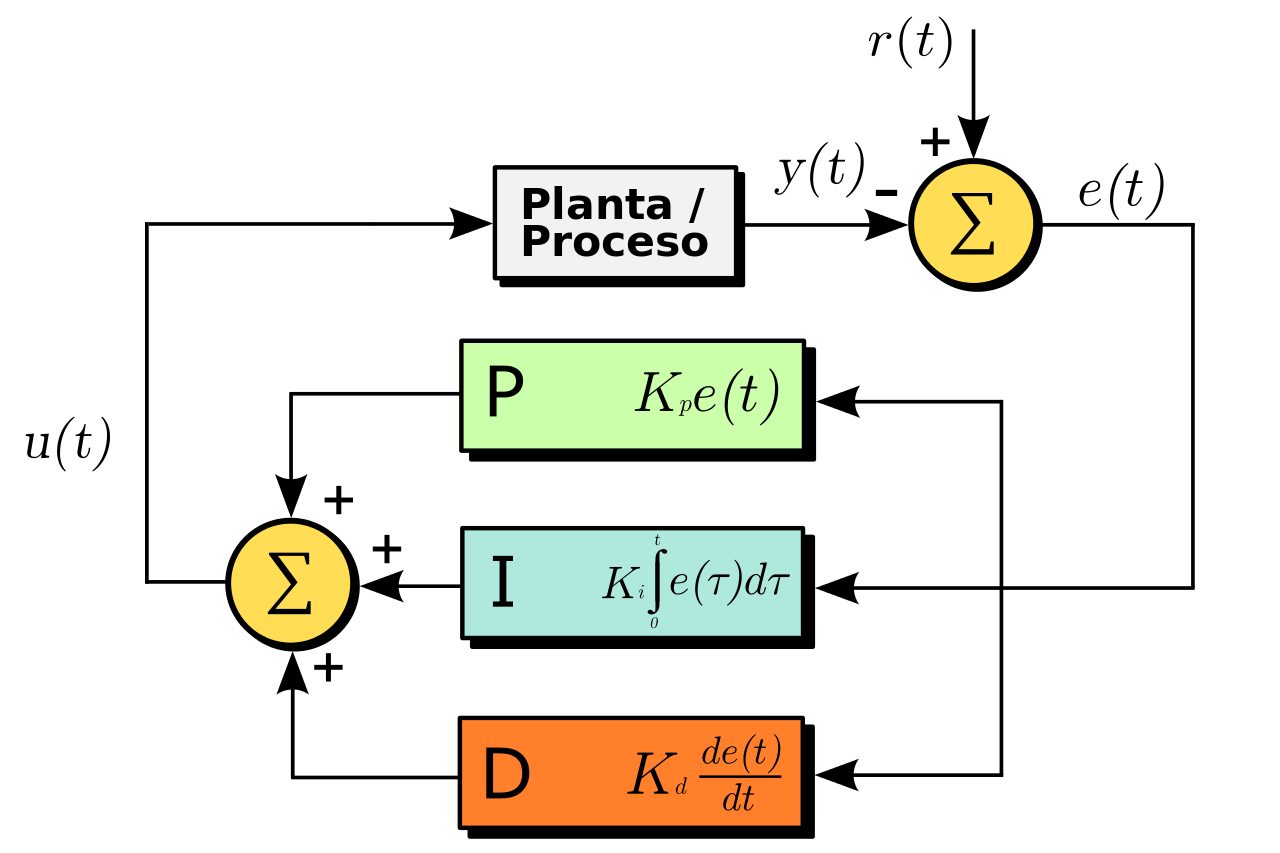
\includegraphics[scale=0.45]{Imagenes/PID_wiki}
\par\end{centering}
\caption{Esquema en bloques del controlador PID.}
\end{figure}
\par\end{center}

\section{Simulaci�n}

\section{Implementaci�n y resultados}

\section{Conclusi�n}
\end{document}
